\subsection{Object-sorting: (fully) relational sequence-to-sequence tasks}\label{ssec:experiments_object_sorting}

In the following set of experiments, we consider sequence-to-sequence relational tasks, and compare an Abstractor-supported model to a plain Transformer. We consider the task of \textit{sorting} sequences of randomly permuted random objects. These experiments are ``purely relational'' in the sense that there exists a relation (order) which is a sufficient statistic for solving the task---the features of individual objects beyond this relation are extraneous. This is a more controlled setting which tests the hypothesis that the inductive biases of the Abstractor indeed confer benefits in modeling relations. We consider the more ``realistic'' setting of partially-relational tasks in the next section. The experiments in the present section demonstrate that the Abstractor enables a dramatic improvement in sample-efficiency on sequence-to-sequence relational tasks.
\begin{figure}[ht]
    \begin{subfigure}[t]{0.40\textwidth}
        %\centering
        \hskip-.35in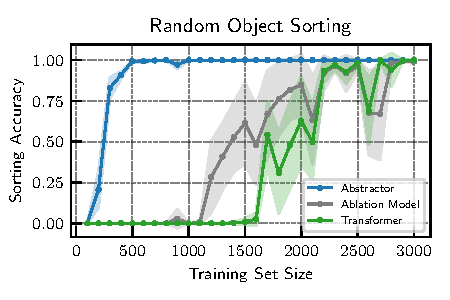
\includegraphics[scale=.95]{figures/experiments/random_object_sorting.pdf}
        \vskip-5pt
        \caption{Learning curves on sorting sequences of random objects. The abstractor is dramatically more sample-efficient.}\label{fig:exp_object_sorting}
    \end{subfigure}\hspace{\fill}
    \begin{subfigure}[t]{0.40\textwidth}
        %\centering
        \hskip-.6in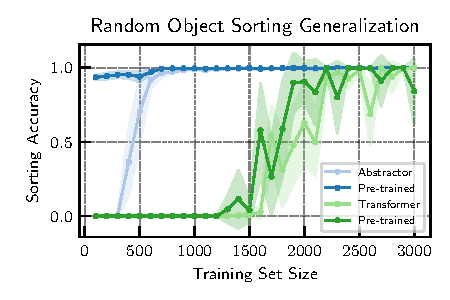
\includegraphics[scale=.95]{figures/experiments/random_object_sorting_generalization.pdf}
        \vskip-5pt
        \caption{Learning curves with and without pre-training on a similar sorting task. The Abstractor benefits from pre-training.}\label{fig:exp_object_sorting_generalization}
    \end{subfigure}
    % \bigskip
    \caption{Experiments on purely relational sequence-to-sequence tasks.}\label{fig:experiments}
    \vskip-.10in
\end{figure}

\subsubsection{Superior sample-efficiency on relational seq2seq tasks compared to standard transformers}\label{sssec:exp_object_sorting_sample_efficiency}

We generate random objects in the following way. First, we generate two sets of random attributes $\mathcal{A} = \{a_1, a_2, a_3, a_4\}$, $a_i \overset{iid}{\sim} \mathcal{N}(0, I) \in \mathbb{R}^{4}$ and $\mathcal{B} = \{b_1, \ldots, b_{12}\}$, $b_i \overset{iid}{\sim} \mathcal{N}(0, I) \in \mathbb{R}^{8}$. To each set of attributes, we associate the strict ordering relation $a_1 \prec a_2 \prec a_3 \prec a_4$ and $b_1 \prec b_2 \prec \cdots \prec b_{12}$, respectively. Our random objects are formed by the Cartesian product of these two attributes $\mathcal{O} = \mathcal{A} \times \mathcal{B}$, yielding $N = 4 \times 12 = 48$ objects (i.e.: each object in $\mathcal{O}$ is a vector in $\mathbb{R}^{4+8}$ formed by a concatenation of one attribute value in $\mathcal{A}$ and one in $\mathcal{B}$). Then, we associate with $\mathcal{O}$ the strict ordering relation corresponding to the order relation of $\mathcal{A}$ as the primary key and the order relation of $\mathcal{B}$ as the secondary key. i.e.: $(a_i, b_j) \prec (a_k, b_l)$ if $a_i \prec a_k$ or if $a_i = a_k$ and $b_j \prec b_l$.

Given a set of objects in $\mathcal{O}$, the task is to sort it according to $\prec$. More precisely, the input sequences are randomly permuted sequences of $10$ objects in $\mathcal{O}$ and the target sequences are the indices of the object sequences in sorted order (i.e., the `argsort'). The training data are sampled uniformly from the set of length-10 sequences in $\mathcal{O}$. We also generate a non-overlapping validation dataset (used during training for early stopping) and a testing dataset (used during evaluation).

We evaluate learning curves on an Abstractor, a Transformer, and an ``Ablation'' model (10 trials for each training set size). The Abstractor uses the architecture $\texttt{Encoder} \to \texttt{Abstractor} \to \texttt{Decoder}$ (architecture (b) in~\Cref{fig:abstractor_architectures}). The Encoder-to-Abstractor interface uses relational cross-attention and the Abstractor-to-Decoder interface uses standard cross-attention. The Ablation Model aims to test the effects of the relational cross-attention in the Abstractor model---it is architecturally identical to the Abstractor model with the crucial exception that the Encoder-to-Abstractor interface instead uses standard cross-attention. The hyperparameters of the models are chosen so that the parameter counts are similar. % TODO: add details here? or in supplement?
We find that the Abstractor is dramatically more sample-efficient than the Transformer and the Ablation model~(\Cref{fig:exp_object_sorting}).

\subsubsection{Ability to generalize to similar tasks}\label{sssec:exp_object_sorting_generalization}

Continuing with the object-sorting task and the dataset generated as described above, we test the Abstractor's ability to generalize from similar relational tasks through pre-training. The main task uses the same dataset described above. The pre-training task involves the same object set $\mathcal{O}$ but the order relation is changed. The ordering in attribute $\mathcal{A}$ is randomly permuted, while the ordering in attribute $\mathcal{B}$ is kept the same. A strict ordering relation $\prec$ on $\mathcal{O}$ is obtained in the same way---using the order in $\mathcal{A}$ as the primary key and the order in $\mathcal{B}$ as the secondary key.

The Abstractor model here uses the architecture $\texttt{Abstractor} \to \texttt{Decoder}$ (i.e.: no Transformer
encoder), and the transformer is the same as the previous section. We pre-train both models on the pre-training task
and then, using those learned weights for initialization, evaluate learning curves on the original task. Since the
Transformer requires more training samples to learn the object-sorting task, we use a pre-training set size of $3,000$, chosen based on the results of the previous subsection so that it is large enough for the Transformer to learn the pre-training task. This experiment assesses the models' ability to generalize relations learned on one task to a new task.~\Cref{fig:exp_object_sorting_generalization} shows the learning curves for each model with and without pre-training. We observe that when the Abstractor is pre-trained, its learning curve on the object-sorting task is significantly accelerated. The transformer does not benefit from pre-training.
